\section{Background and Theory}
\label{sec:background}


\subsection{Overview}
\label{subsec:background_overview}
This section covers the mathematical and theoretical foundations of the project. Section~\ref{subsec:background_statistic} and Section~\ref{subsec:background_regression} outline the mathematical and regression principles used. Section~\ref{subsec:background_model_loss_decomposition} and Section~\ref{subsec:background_ensemble_learning} explain the benefits of ensemble learning over a single model. Section~\ref{subsec:background_ncl} extends from it and motivates the study of a particular ensemble learning technique (\textit{NCL}). Finally, Section~\ref{subsec:background_neat} covers NEAT, which is used for the NCL-extension discussed in Section~\ref{subsec:stage_4}. 


\subsection{Statistical Foundations}
\label{subsec:background_statistic}
\begin{theorem}[Law of Large Numbers]\label{theorem:law_of_large_numbers}
    As sample size grows, the empirical average becomes more consistent and stays closer to the true mean. 
\end{theorem}
See~\cite{durrett2019probability}~\cite{judd1985law} for its motivations and proofs. Theorem~\ref{theorem:law_of_large_numbers} helps explain certain behaviours due to different ensemble size $m$ in Section~\ref{subsubsec:evaluation_neat_ncl_observations}. 


\subsection{Regression in supervised learning}
\label{subsec:background_regression}
Supervised learning utilises labeled datasets to train models for pattern recognition and outcome prediction. This project specifically addresses regression tasks, characterised by continuous numerical outputs. Since these models target known values, various performance metrics are used to quantify the accuracy of their predictions: 
\begin{equation}
    \label{equation:mse}
    MSE = \frac{1}{m} \sum_{i=1}^{m} (\hat{y}_i - y)^{2}
\end{equation}
\begin{equation}
    \label{equation:rmse}
    RMSE = \sqrt{\frac{1}{m} \sum_{i=1}^{m} (\hat{y}_i - y)^{2}}
\end{equation}
This project employs MSE (Equation~\ref{equation:mse}). Equation~\ref{equation:rmse} is also used to evaluate performance in Section~\ref{subsubsec:evaluation_baseline_observations}. 


\subsection{Model Loss Decomposition}
\label{subsec:background_model_loss_decomposition}
Theorem~\ref{theorem:bias_variance_decomposition} decomposes the expected error of a learner into three distinct terms, illustrating that model performance is fundamentally a trade-off between bias and variance: 
\begin{theorem}[Bias-variance Decomposition]\label{theorem:bias_variance_decomposition}
    Given a learning algorithm that produces a predictor (its prediction is $\hat{y}$) from a random training set $\mathcal{S}$, the expected risk is given as (assume squared loss is used): 
    \begin{align*}
        \underbrace{\mathbb{E}_{\mathcal{S}}\left[\mathbb{E}_{\mathbf{x}y}\left[(y - \hat{y})^2\right]\right]}_{\text{expected risk}} = \underbrace{\mathbb{E}_{\mathbf{x}y}\left[(y - \hat{y^*})^2\right]}_{\text{noise}} + \underbrace{\mathbb{E}_{\mathbf{x}y}\left[\left(\hat{y^*} - \mathbb{E}_{\mathcal{S}}[\hat{y}]\right)^2\right]}_{\text{bias}} + \underbrace{\mathbb{E}_{\mathbf{x}y}\left[\mathbb{E}_{\mathcal{S}}\left[(\hat{y} - \mathbb{E}_{\mathcal{S}}[\hat{y}])^2\right]\right]}_{\text{variance}}
    \end{align*}
\end{theorem}
See~\cite{geman1992neural} for proof. Theorem~\ref{theorem:bias_variance_decomposition} allows the analysis of \textit{why} a model is failing. In underfitting, the model assumptions are too rigid to capture the underlying pattern (high bias). In overfitting, the model is too flexible and treats random noise in the training data as a genuine pattern (high variance). It also states the theoretical limit that no model can ever be perfect and $\mathbb{E}_{\mathbf{x}y}\left[(y - \hat{y^*})^2\right]$ represents the irreducible error. 


\subsection{What is ensemble learning? }
\label{subsec:background_ensemble_learning}
Instead of training a single model in traditional supervised learning, \textbf{ensemble learning} involves training a ``committee'' of models (i.e. \textit{base learners}). While common algorithms include Bagging~\cite{breiman1996bagging}, Boosting~\cite{freund1997decision} and Mixture of Experts~\cite{jacobs1991adaptive}, this project explores NCL (Section~\ref{subsec:background_ncl}), which actively encourages diversity among base learners while focusing on individual accuracy. 

One major advantage of ensemble learning is that the ensemble population risk is mathematically bounded by the average population risk of all base learners: 
\begin{theorem}\label{theorem:ensemble_population_risk_le_average_population_risk}
    When squared loss is used, 
    \begin{align*}
        R(\bar{y}) \le \frac{1}{m} \sum_{i=1}^{m} R(\hat{y}_i)
    \end{align*}
\end{theorem}
See~\cite{krogh1994neural} for proof. While population risk is not something measurable as it requires infinite amount of data, Theorem~\ref{theorem:ensemble_population_risk_le_average_population_risk} still provides a strong theoretical foundation for the benefits and motivations of ensemble learning. Consistent with Theorem~\ref{theorem:ensemble_population_risk_le_average_population_risk}, the empirical ensemble loss is mathematically bounded by the average loss of all base learners as the ambiguity term is always non-negative: 
\begin{theorem}[Ambiguity Decomposition]\label{theorem:ambiguity_decomposition}
    When squared loss is used, 
    \begin{align*}
        \underbrace{(y - \bar{y})^2}_{\text{ensemble loss}} = \underbrace{\frac{1}{m} \sum_{i=1}^{m} (\hat{y}_i - y)^2}_{\text{average loss}} - \underbrace{\frac{1}{m} \sum_{i=1}^{m} (\hat{y}_i - \bar{y})^2}_{ambiguity}
    \end{align*}
\end{theorem}
See~\cite{krogh1994neural} for proof. The ambiguity term is $0$ only if every base learner produces identical predictions, i.e. $\hat{y}_i = \bar{y}$, and the ensemble will offer no advantage over a single MLP. In practice, $m$ identical predictions are not likely because every base learner is trained with a separate randomly-shuffled dataset, converging to different weights even if other hyperparameters are set the same. Thus, an ensemble model is no worse than a single model. 

Diversity has a major role in the performance improvement of an ensemble model. Increased diversity directly reduces the expected ensemble error: 
\begin{theorem}[Bias-variance-diversity Decomposition]\label{theorem:bias_variance_diversity_decomposition}
    For a set of models combined as an arithmetic mean $\hat{y}_{ensemble} = \bar{y} = \frac{1}{m} \sum_{i=1}^{m} \hat{y}_i$, the expected risk of the ensemble admits the following decomposition (assume squared loss is used): 
    \begin{align*}
        \underbrace{\mathbb{E}_{\mathcal{S}}\left[\mathbb{E}_{\mathbf{x}y}\left[(y - \bar{y})^2\right]\right]}_{\text{expected ensemble risk}} = 
        \\
        &\phantom{=} \underbrace{\mathbb{E}_{\mathbf{x}y}\left[(y - \hat{y^*})^2\right]}_{\text{noise}} + \underbrace{\frac{1}{m} \sum_{i=1}^{m} \mathbb{E}_{\mathbf{x}y}\left[\left(\hat{y^*} - \mathbb{E}_{\mathcal{S}}[\hat{y}_i]\right)^2\right]}_{\text{average bias}} + \underbrace{\frac{1}{m} \sum_{i=1}^{m} \mathbb{E}_{\mathbf{x}y}\left[\mathbb{E}_{\mathcal{S}}\left[(\hat{y}_i - \mathbb{E}_{\mathcal{S}}[\hat{y}_i])^2\right]\right]}_{\text{average variance}}
        \\
        &\phantom{=}  - \underbrace{\mathbb{E}_{\mathbf{x}y}\left[\mathbb{E}_{\mathcal{S}}\left[\frac{1}{m} \sum_{i=1}^{m} (\hat{y}_i - \bar{y})^2\right]\right]}_{\text{diversity}}
    \end{align*}
\end{theorem}
It is derived by first applying Theorem~\ref{theorem:ambiguity_decomposition} to $\mathbb{E}_{\mathcal{S}}\left[\mathbb{E}_{\mathbf{x}y}\left[(y - \bar{y})^2\right]\right]$ in Theorem~\ref{theorem:bias_variance_diversity_decomposition} followed by Theorem~\ref{theorem:bias_variance_decomposition}. See~\cite{brown2005managing} for another proof. The diversity term in Theorem~\ref{theorem:bias_variance_diversity_decomposition} can be thought as the expected value of the ambiguity term in Theorem~\ref{theorem:ambiguity_decomposition} over all training datasets $\mathcal{S}$ and all input data $\mathbf{x}$. It is measusred using diversity coefficient (Equation~\ref{equation:diversity_coefficient}), which is the variance of ensemble predictions (another representation of the ambiguity term in Equation~2 of Krogh and Vedelsby~\cite{krogh1994neural}): 
\begin{equation}
    \label{equation:diversity_coefficient}
    \rho = \frac{1}{m} \sum_{i=1}^{m} (\hat{y}_i - \bar{y})^{2}
\end{equation}
Even if average loss remains unchanged, increasing the number of base learners makes diverse predictions more likely. This happens because each learner is trained on a different randomly-shuffled dataset, leading to greater ambiguity (distance from mean prediction) and lower ensemble error. Theorem~\ref{theorem:bias_variance_diversity_decomposition} illustrates how diversity reduces ensemble error, highlighting the core objective of this project. 


\subsection{What is Negative Correlation Learning? }
\label{subsec:background_ncl}
An ensemble learning method called \textbf{Negative Correlation Learning} (NCL) is explored in this project. Unlike traditional approaches such as Bagging~\cite{breiman1996bagging} and Boosting~\cite{freund1997decision}, which do not change the loss function and promote diversity through data sub-sampling and re-weighting, NCL enforces diversity actively by adding a penalty term to loss function of each base learner. The complete loss function of NCL is given below: 
\begin{equation}
    \label{equation:ncl}
    \underbrace{\mathcal{L}_i}_{\text{ith base learner loss}} = \underbrace{(\hat{y}_i - y)^2}_{\text{squared loss of 1 data point}} - \lambda \underbrace{(\hat{y}_i - \bar{y})^2}_{\text{correlation penalty function}}
\end{equation}
Correlation penalty function assigns a high penalty when base learners are positively correlated (nearly identical predictions). By systematically penalising high similarity, NCL forces the base learners to explore a broader hypothesis space, leading to more diverse individual predictions. Minimising this loss function involves a dual objective: minimising $(\hat{y}_i - y)^2$ to ensure each base learner maintains high predictive accuracy while maximising the penalty term $(\hat{y}_i - \bar{y})^2$ promotes functional deviation of learners' predictions from mean prediction $\bar{y}$. The correlation penalty coefficient $\lambda$ regulates this trade-off. As $\lambda$ increases, the optimisation process places greater weight on prediction diversity. This theoretical expectation suggests that higher $\lambda$ values will directly result in a more heterogeneous committee of learners, maximising the ambiguity term in Theorem~\ref{theorem:ambiguity_decomposition} (and diversity term in Theorem~\ref{theorem:bias_variance_diversity_decomposition}). 

While $\lambda$ is typically set within $[0, 1]$, its upper bound (given by Equation~\ref{equation:lambda_upper_bound}) can be larger than $1$ under certain conditions~\cite{brown2005managing}, e.g. when $m = 2$: 
\begin{equation}
    \label{equation:lambda_upper_bound}
    \lambda_{upper\_bound} = \frac{m^2}{2(m - 1)^2}
\end{equation}
In this project, $(\hat{y}_i - y)^2$ is averaged across all data points, making it the same as the PyTorch MSE used. From Equation~\ref{equation:lambda_upper_bound}, the upper bound of $\lambda$ decreases as $m$ grows: 
\begin{enumerate}
    \item \textbf{For $m = 2$, } \\
    $\lambda_{upper\_bound} = 2.0$

    \item \textbf{For $m = 6$, } \\
    $\lambda_{upper\_bound} = 0.72$

    \item \textbf{For $m = 12$, } \\
    $\lambda_{upper\_bound} \approx 0.595$
\end{enumerate}

Interestingly, the ensemble changes its behaviour based on the accuracy-diversity trade-off via changing $\lambda$. When $\lambda = 0$, the penalty term $p_i$ disappears and the loss function reverts to squared loss. Base learners are trained independently and no active diversity is encouraged. When $0 < \lambda < \lambda_{upper\_bound}$, the model balances individual performance with ensemble diversity. From Theorem~\ref{theorem:ambiguity_decomposition} and Theorem~\ref{theorem:bias_variance_diversity_decomposition}, increasing diversity should theoretically reduce the overall ensemble risk. When $\lambda = 1$, a unique case occurs (Theorem~\ref{theorem:loss_function_ncl_lambda_1}), where the loss function no longer depends on the index of the $i$th base learner, effectively treating the entire ensemble as a single unified estimator, i.e. $\hat{y}_{ensemble} = \bar{y}$: 
\begin{theorem}\label{theorem:loss_function_ncl_lambda_1}
    For ith base learner, when MSE is used and the ensemble model uses an arithmetic-mean-aggregator, the average loss of the ith base learner across all $n$ data points (when $\lambda = 1$) is given below: 
    \begin{align*}
        \underbrace{\mathcal{L}_i}_{\text{ith base learner loss}} = \frac{1}{n} \sum^{n}_{i = 1} \underbrace{(\bar{y} - y)^2}_{\text{squared loss of 1 data point}}
    \end{align*}
\end{theorem}
See~\cite{brown2003negative} for proof. Lastly, when $\lambda > \lambda_{upper\_bound}$, the emphasis on diversity overrides the requirement for individual accuracy, resulting in a deterioration of performance and an increase in ensemble risk. 

Proposed by Liu et al.\ \cite{liu1999ensemble}, the loss function of the $i$th base learner is $\mathcal{L}_i = \frac{1}{2} (\hat{y}_i - y)^2 - \lambda p_i$, where $p_i$ penalises similarity between predictions. The initial formula assumed $p_i = (\hat{y}_i - \bar{y}) \sum_{j \neq i} (\hat{y}_j - \bar{y})$, with $\bar{y}$ treated as a constant with respect to $\hat{y}_i$. Based on this assumption, Theorem~\ref{theorem:ncl_differentiation_incorrect} was proposed~\cite{liu1999ensemble}: 
\begin{theorem}\label{theorem:ncl_differentiation_incorrect}
    When $\bar{y}$ is assumed to have a constant value with respect to $\hat{y}_i$, the derivative of $p_i$ with respect to $\hat{y}_i$ is given below: 
    \begin{align*}
        \frac{\partial{p_i}}{\partial{\hat{y}_i}} = -(\hat{y}_i - \bar{y})
    \end{align*}
\end{theorem}
See~\cite{liu1999ensemble} for proof. This assumption was later shown to be incorrect~\cite{brown2005managing}. Consequently, the penalty term was revised to $p_i = -(\hat{y}_i - \bar{y})^2$ (see ~\cite{brown2003negative}) with an updated derivation given in Theorem~\ref{theorem:ncl_differentiation_correct}: 
\begin{theorem}\label{theorem:ncl_differentiation_correct}
    When $\bar{y}$ is not assumed to have a constant value with respect to $\hat{y}_i$, the derivative of $p_i$ with respect to $\hat{y}_i$ is given below: 
    \begin{align*}
        \frac{\partial{p_i}}{\partial{\hat{y}_i}} = \frac{-2 (m - 1)}{m} (\hat{y}_i - \bar{y})
    \end{align*}
\end{theorem}
, where $m$ is the ensemble size. 
\\
See~\cite{brown2005managing} for proof. This revision affected the upper bound of $\lambda$. From Brown et al.\ \cite{brown2005managing}, $\lambda_{upper\_bound} = \frac{m}{m - 1}$ under an independence assumption between $\bar{y}$ and $\hat{y}_i$. Otherwise, $\lambda_{upper\_bound} = \frac{m^2}{2(m - 1)^2}$. This project adopts the latter. 


\subsection{What is NeuroEvolution of Augmenting Topologies? }
\label{subsec:background_neat}
\textbf{NeuroEvolution of Augmenting Topologies} (NEAT)~\cite{stanley2002evolving} is a genetic algorithm-based method~\cite{miller1989designing} for evolving neural networks. Unlike standard approaches that utilise a fixed architecture, NEAT evolves both weights and topologies by dynamically adding or removing nodes and connections while employing speciation to protect structural innovations. The hierarchy of a NEAT base learner is represented as a directed graph of nodes and edges. While traditional NEAT is fundamentally an evolutionary algorithm and does not utilise gradient-based optimisation~\cite{rumelhart1986learning}, it is still suitable to problems involving feedforward neural network~\cite{montana1989training}, making NEAT already suitable for this project. In fact, this project integrates NEAT with NCL and incorporates gradient descent to refine network parameters. 

\subsubsection{NEAT Notation and Terminology}
The following definitions establish the core NEAT terminology used in this report: 

\paragraph{Genome} is the encoded representation of a neural network, analogous to its ``DNA''. While various methods exist (e.g. bit-string representation~\cite{schaffer1992combinations}, indirect encoding~\cite{stanley2009hypercube}, graph encoding~\cite{kitano1990designing}~\cite{pujol1998evolving} etc.), this project utilises a specific form of graph encoding(refer to~\cite{McIntyre_neat-python} for its open-source repository) to more naturally reflect the network topology. Within this framework, a genome consists of a directed graph where nodes represent neurons and edges represent weighted connections. 

\paragraph{Phenome} is the functional neural network expressed by its corresponding genome. Utilising a direct encoding scheme, NEAT explicitly represents every structural element such as nodes and edges as a specific gene. Consider genome as the ``DNA'' while phenome as the resulting ``organism''. 

\paragraph{Crossover} is the process of combining 2 parent genomes to produce an offspring genome. There are 3 types of genes: 
\begin{enumerate}
    \item \textit{Matching Gene} \\
    A gene that has the same innovation number and exist in both parent genomes, which will be randomly selected to pass down to the offspring genome. The minimum and maximum innovation numbers of all matching genes form the \textit{shared historical range}. 

    \item \textit{Disjoint Gene} \\
    A non-matching gene within the shared historical range that appears in 1 parent genome only. Disjoint genes of the less-fit parent genome are ignored during crossover. 

    \item \textit{Excess Gene} \\
    A non-matching gene beyond the shared historical range that appears in 1 parent genome only. Excess genes of the less-fit parent genome are ignored during crossover. 
\end{enumerate}

Figure~\ref{fig:background_neat_crossover} illustrates a NEAT crossover between two parent genomes. In this example, the phenome processes three input features (nodes~1-3) to produce a single output (node~4), with bold arrows indicating the direction of data flow. 
Each gene is represented by a rectangle detailing its innovation number, connection node IDs and activation status. Blue and green backgrounds identify genes from Parent~1 and Parent~2 respectively. 
During crossover, genes are aligned by their innovation numbers: 
\begin{enumerate}
    \item Matching Gene \\
    Randomly selected from either parent. 

    \item Disjoint and Excess Gene \\
    Inherited solely from the more fit parent (Parent~2) while those from the less fit parent (Parent~1) are skipped. 
\end{enumerate}

Within the shared historical range $[1, 7]$, genes~4, 8 and 9 from Parent~1 are ignored. Consequently, the resulting offspring primarily inherits its genetic structure from the more fit parent. 

% 1 Image
\begin{figure}[H]
    \capstart
    \centering
    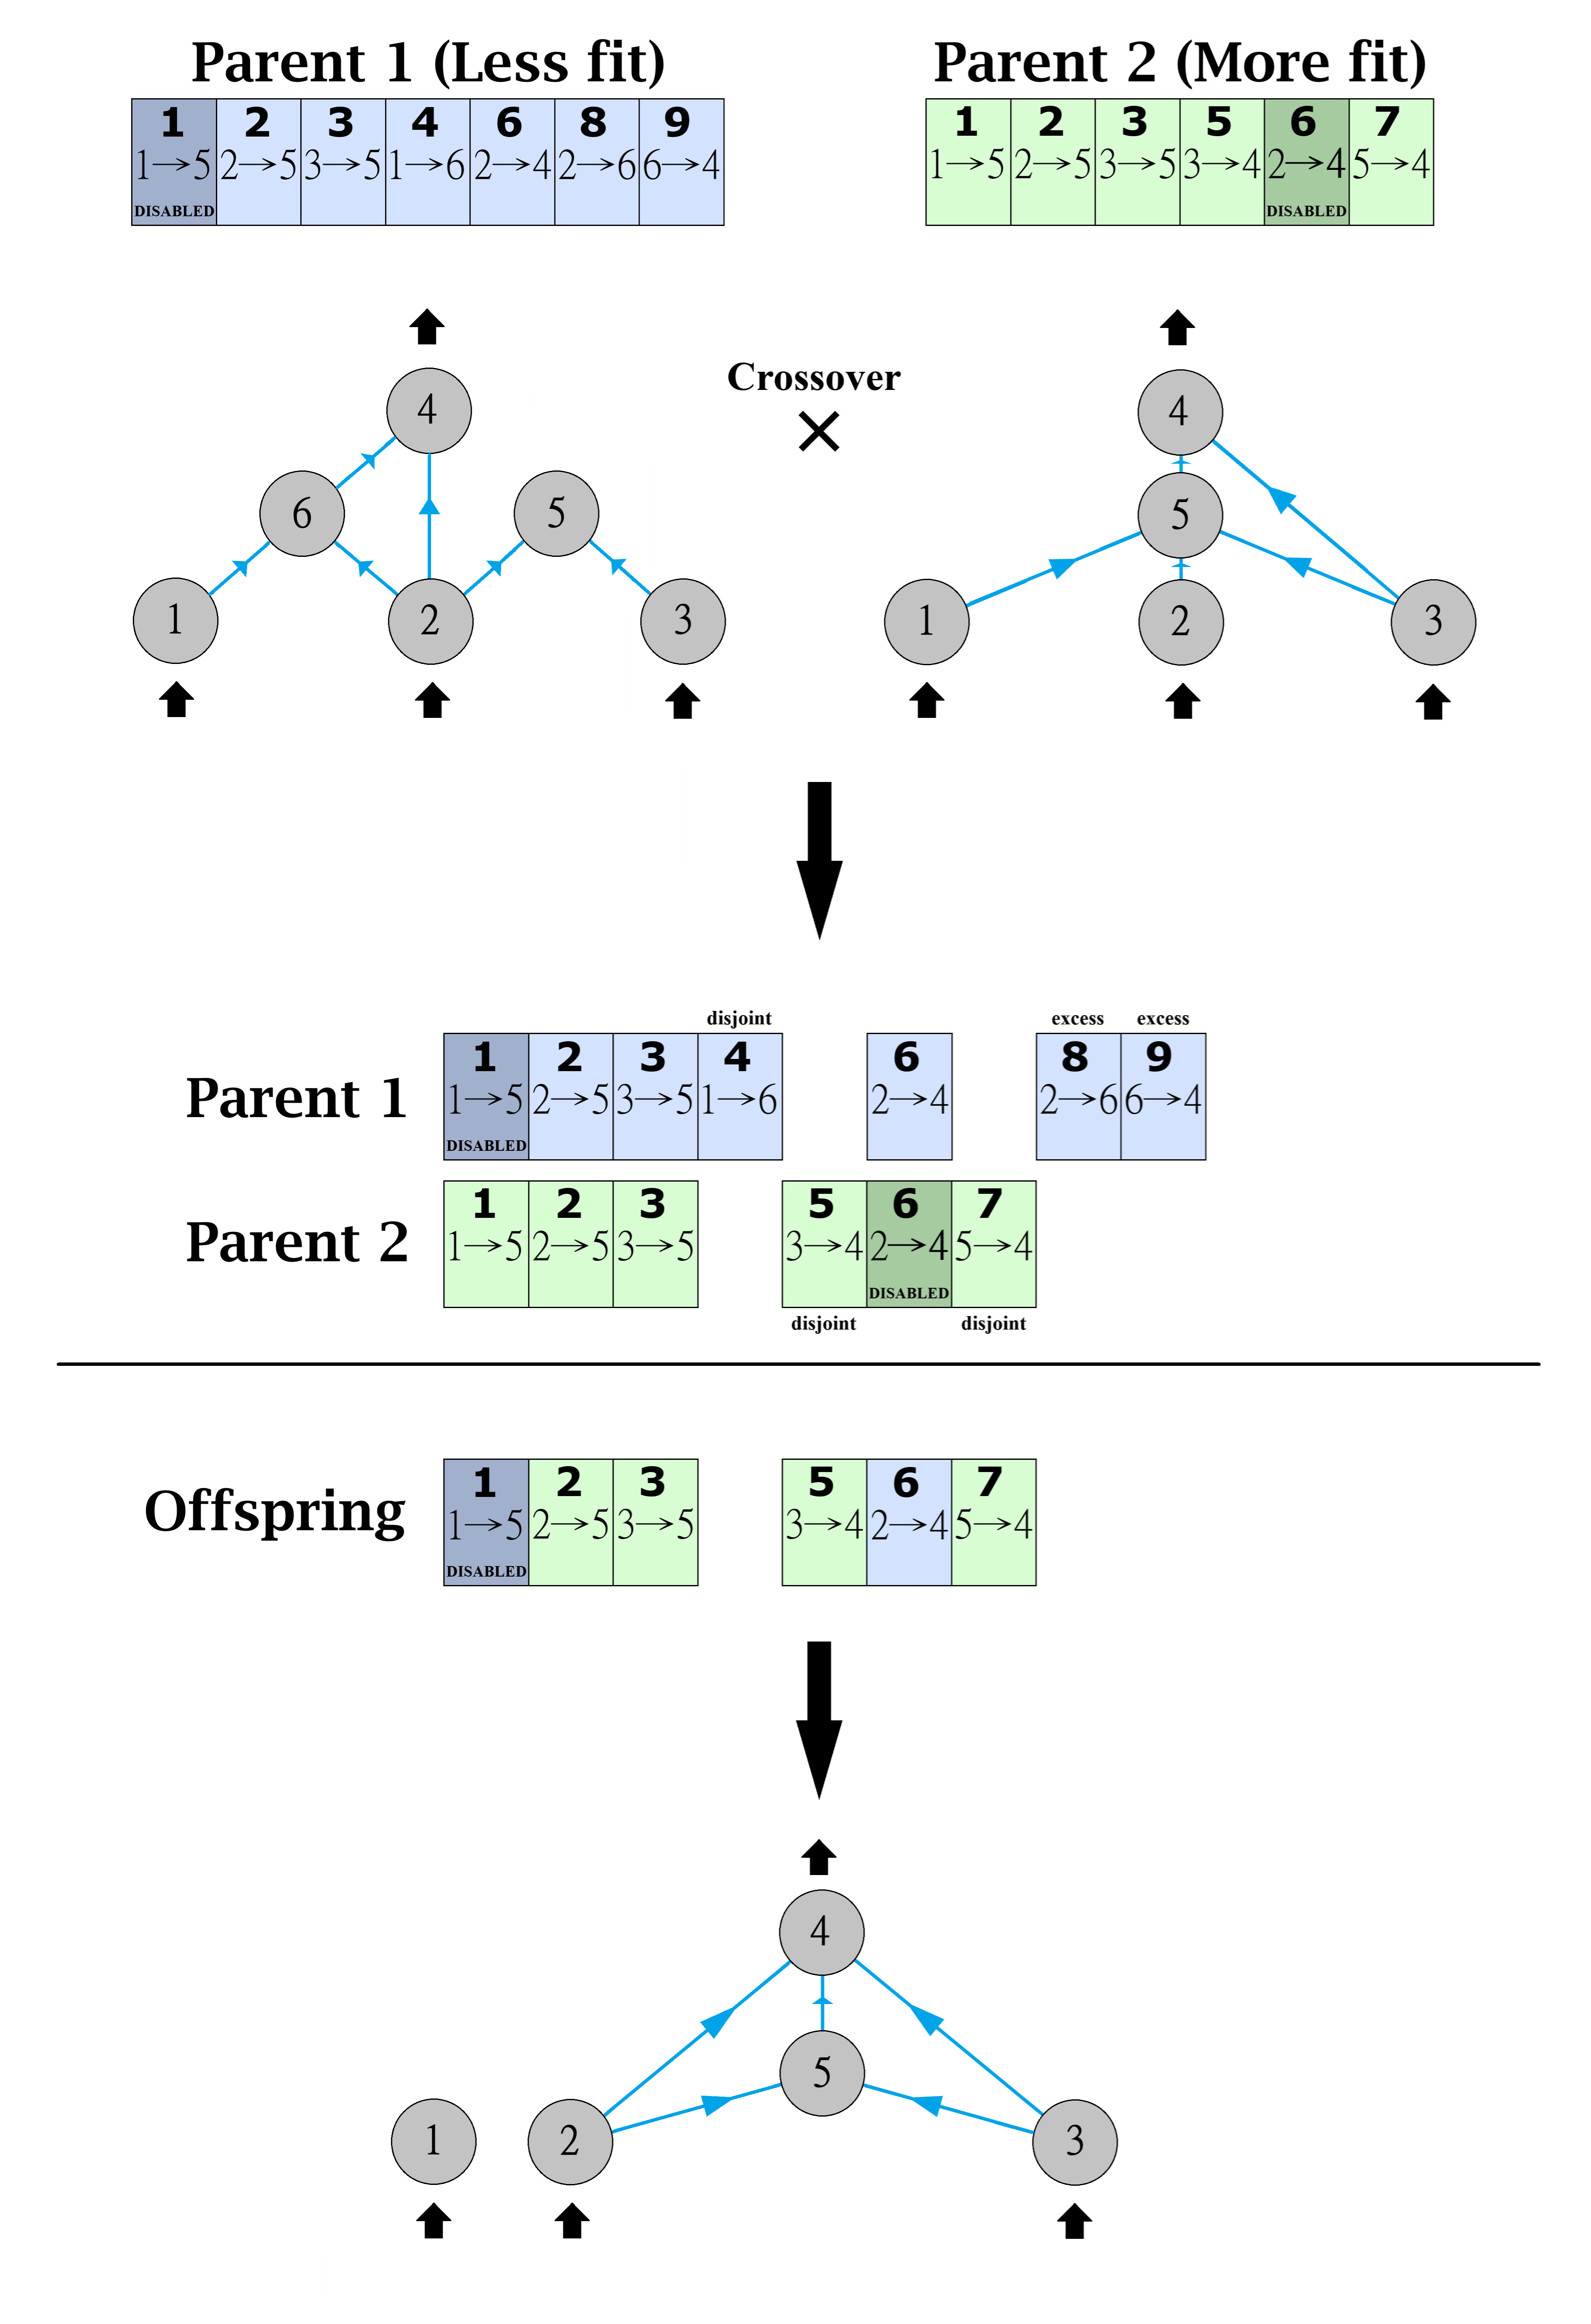
\includegraphics[width=0.64\textwidth]{img/background/neat-crossover.png}
    \caption{Example of NEAT crossover between 2 parent genomes}
    \label{fig:background_neat_crossover}
\end{figure}

\paragraph{Speciation} partitions the population into distinct groups based on topological similarity, enabling networks to compete primarily within their own \textit{species} (a subgroup of genetically similar genomes). This mechanism protects structural innovation by ensuring that nascent, lower-fitness genomes are not prematurely outcompeted by established, high-fitness individuals. Protection is further maintained by setting an appropriate \textit{elitism} threshold within each species. 

\paragraph{Innovation number} is a globally unique identifier assigned to each new node or connection created through mutation. It tracks the origin of genetic features and identifies homologous genes across structurally diverse networks. It facilitates efficient, meaningful recombination (e.g. during crossover) without the need for complex topological mapping. 

\paragraph{Genetic distance} (also known as \textit{compatibility distance}) is the metric used to quantify the similarity between two genomes for speciation. Defined in Equation~\ref{equation:neat_ncl_genetic_distance}, it incorporates (potentially with different weightings) the number of excess and disjoint genes and the average weight differences between matching genes. 

\paragraph{Elitism} is a mechanism to ensure the best individuals within a species (more common)/population (less common) can survive to the next generation. Normally, the next generation is created via mutation and crossover. However, due to randomness, some best genomes might be lost. Elitism protects few exceptional, ``elite'' genomes by carrying them over unchanged without the normal competition for reproduction. The number of ``elite'' genomes can be set by developers. 

\paragraph{Stagnation} is the situation where a species stops improving in their fitness levels over some generations, i.e. it becomes \textit{stagnant}. Stagnant species are eventually removed from the population to focus resources on more promising species. 

\paragraph{Mutation} is a process of introducing random changes to genomes via adjusting connection weight, adding/removing a connection or adding/removing a neuron. Structural mutations allow networks to become more complex over time. 

\paragraph{Fitness} is a score used to measure how well a phenome performs on a given task, which is then used to select which genomes to survive and reproduce to give stronger offsprings. A higher fitness means the phenome is fitter. 

\paragraph{Fitness sharing} is a technique designed to maintain population diversity and prevent premature convergence in Genetic Algorithms. It allows different network topologies to evolve and co-exist without being immediately outcompeted by a single, temporarily superior species. It achieves this by reducing the fitness of similar individuals, effectively enforcing the exploration of different regions of the search space. 

\paragraph{Sharing factor} is a number that quantifies how crowded the species of a genome is. The higher the sharing factor, the more crowded the species is. It is computed based on similarity to other genomes via a distance metric, which can be based on genotypic similarity (e.g. Hamming distance for binary representations~\cite{hamming1950error}) or phenotypic similarity (e.g. Euclidean distance in the solution space). Such calculation is used in fitness sharing to compute the adjusted, final fitness of a phenome by the formula $adjusted\_fitness = \frac{raw\_fitness}{sharing\_factor}$ before selection for the next generation. 

\paragraph{Niche radius} ($\sigma$) is a threshold value used to determine whether two phenomes are considered close/similar enough to share fitness. It is usually a hyperparameter set by developers but in Section~\ref{subsec:stage_4}, it is computed dynamically. 


\subsubsection{Steps of traditional NEAT evolutionary algorithm}
\begin{enumerate}
    \item \textbf{Initialisation} \\
    The process starts by generating an initial population of candidate solutions. They are generated randomly and are typically represented as a genome with encoded features and characteristics. 

    \item \textbf{Evaluation} \\
    Each candidate solution is evaluated how well it solves the given problem using a fitness function, which assigns a numerical score to each solution. When fitness sharing is enabled, the raw fitness is updated considering sharing factor. The adjusted fitness is used for the next step. 

    \item \textbf{Selection} \\
    Based on the calculated fitness, a subset of the population is selected to become the ``parents'' of the next generation. Individuals with higher fitness scores have a higher probability of being selected to encourage the reproduction of stronger offsprings. 

    \item \textbf{Reproduction} \\
    The selected individuals then reproduce to create ``offspring'' for the next generation using two genetic operators, crossover and mutation. 

    \item \textbf{Replacement} \\
    The newly generated offspring replaces the current population (either entirely or partially), forming the new generation. If elitism is enabled, $n$ (specified by developers) ``elite'' genomes are copied directly to the next generation without modification. 

    \item \textbf{Termination} \\
    Steps 2-5 are repeated until one of the two conditions is met: a certain fitness threshold (specified by developers) is reached (i.e. a satisfactory solution is found) or the maximum number of generations is reached. 
\end{enumerate}


\subsection{Graph algorithms}


\subsubsection{Topological sort}
Topological sort is a linear ordering of nodes in a Directed Acyclic Graph (DAG) where for every directed edge \texttt{(node\_start, node\_end)}, \texttt{node\_start} comes before \texttt{node\_end}. It is used to schedule tasks with dependencies and is used in Section~\ref{subsubsec:dynamic_nn_on_gpu}. 
Below contains the pseudo-code of the algorithm: 

\begin{lstlisting}[language=Python, caption={Depth-first search used in topological sort}]
function depth_first_search(node: Node, nodes_in_topological_sort: [Node]):
    # Get the state of this node: 
    # 'N' - New node that has not been explored
    # 'O' - Open node whose successors are currently being explored
    # 'F' - Finished node whose all successors have been explored
    node_state = get_state(node)

    if node_state == 'N':
        # Mark this node as 'O'
        set_state(node, 'O')
    else if node_state == 'O':
        # Cycle is detected
        # Error is raised because a DAG is expected in order to find a topological sort
        raise Error("Detected cycle in the graph")
    else if node_state == 'F':
        # This node has been explored so we do nothing
        pass
    else:
        # Invalid node_state
        raise Error("Invalid node_state (expect 'N'/'O'/'F')")
    
        for successor in node.successors:
            # successor is a child node of the current node
            depth_first_search(successor, nodes_in_topological_sort)
        
        # All successors of the current node have been explored
        # Mark the current node as 'F'
        set_state(node, 'F')

        # Prepend the current node to the beginning of the list of nodes in topological sort
        nodes_in_topological_sort.prepend(node)
\end{lstlisting}

\begin{lstlisting}[language=Python, caption={Topological sort}]
function topological_sort(nodes: [Node]):
    # A list of nodes in topological sort
    nodes_in_topological_sort = []

    # Set all nodes to their initial states 'N'
    for n in nodes:
        set_state(n, 'N')
    
    # Get all starting nodes in the DAG
    start_nodes = find_all_start_nodes(nodes)

    for start_node in start_nodes:
        # Error checking to make sure a start node retrieved from findl_all_start_nodes(nodes) has the correct state
        assert get_state(start_node) == 'N'

        depth_first_search(start_node, nodes_in_topological_sort)
    
    return nodes_in_topological_sort
\end{lstlisting}